\chapter{Design of a malicious eBPF rootkit}
In the previous chapter, we discussed the capabilities of eBPF programs from a security standpoint, detailing which helpers and program types are particularly useful for developing malicious programs, and analysing some techniques (stack scanning, overwriting packets together with TCP retransmissions) which helps us circumvent some of the limitations of eBPF.

Taking as a basis these capabilities, this chapter is now dedicated to a comprehensive description of our rootkit, including the techniques and functionalities implemented, thus showing how these capabilities can lead to the creation of a real malicious application. As we mentioned during the project objectives, our goals for our rootkit include the following:
\begin{itemize}
\item Hijacking the execution of user programs while they are running, injecting libraries and executing malicious code, without impacting their normal execution.
\item Featuring a command-and-control module powered by a network backdoor, which can be operated from a remote client. This backdoor should be controlled with stealth in mind, featuring similar mechanisms to those present in rootkits found in the wild.
\item Tampering with user data at system calls, resulting in running malware-like programs and for other malicious purposes.
\item Achieving stealth, hiding rootkit-related files from the user.
\item Achieving rootkit persistence, the rootkit should run after a complete system reboot.
\end{itemize}

We will firstly present an overview on the rootkit architecture and design. Afterwards, we will be exploring each functionality individually, offering a comprehensive view on how each of the systems work.

\section{Rootkit architecture}
%TODO
\begin{figure}[htbp]
	\centering
	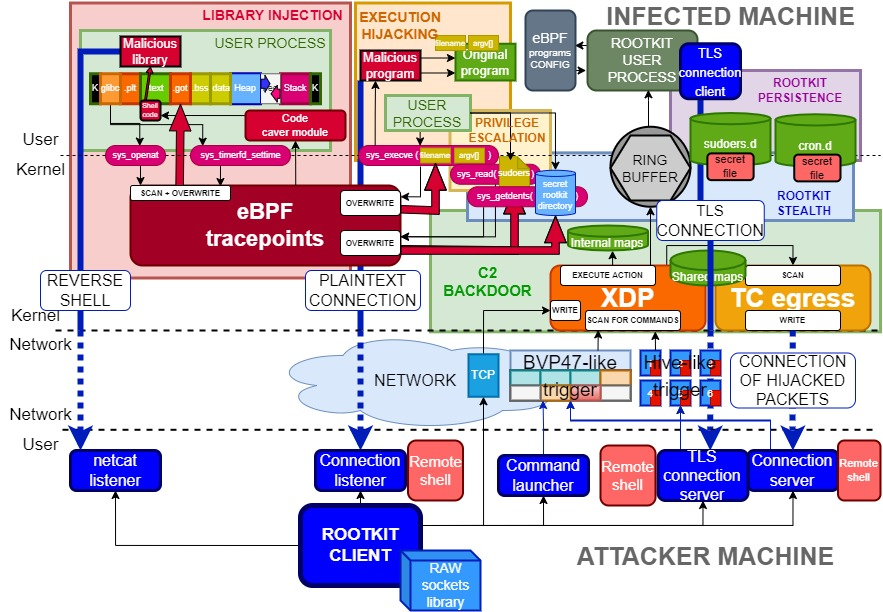
\includegraphics[width=15.5cm]{rootkit.jpg}
	\caption{Overview of the rootkit subsystems and components.}
	\label{fig:rootkit}
\end{figure}


\section{Library injection attacks}
In this section, we will discuss how to hijack an user process running in the system so that it executes arbitrary code instructed from an eBPF program. For this, we will be injecting a library which will be executed by taking advantage of the fact that the GOT section in ELFs is flagged as writable (as we introduced in section \ref{subsection:elf_lazy_binding} and using the stack scanning technique covered in section \ref{subsection:bpf_probe_write_apps}. This injection will be stealthy (it must not crash the process), and will be able to hijack privileged programs such as systemd, so that the code is executed as root.

We will also research how to circumvent the protections which modern compilers have set in order to prevent similar attacks (when performed without eBPF).

This technique has some advantages and disadvantages to the one described by Jeff Dileo at DEFCON 27\cite{evil_ebpf_p6974}, which we will briefly cover before presenting ours. Both techniques will be later compared in section \ref{TODO EVALUATION}.


\subsection{ROP with eBPF} \label{subsection:rop_ebpf}
In 2019, Jeff Dileo presented in DEFCON 27 the first technique to achieve arbitrary code execution using eBPF\cite{evil_ebpf_p6974}. For this, he used the ROP technique we described in section \ref{subsection:rop} to inject malicious code into a process. We will present an overview on his technique, in order to later compare it to the one we will develop for our rootkit, and find advantages and disadvantages. Note that this is a summary and some aspects have been simplified, however we will go in full detail during the explanation of our own technique.

\begin{figure}[H]
	\centering
	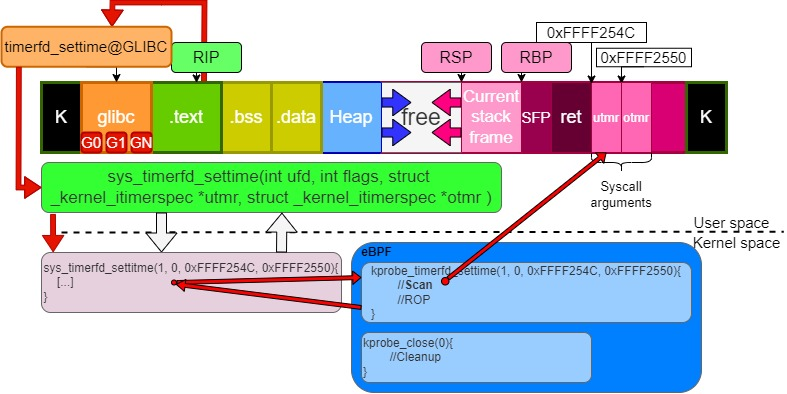
\includegraphics[width=15cm]{rop_evil_ebpf_1.jpg}
	\caption{Initial setup for the ROP with eBPF technique.}
	\label{fig:rop_evil_ebpf_1}
\end{figure}

Figure \ref{fig:rop_evil_ebpf_1} shows an overview on the process memory and the eBPF programs loaded. For this injection, we will use the stack scanning technique (section \ref{subsection:bpf_probe_write_apps}) using the arguments of a system call whose arguments are passed using the stack (sys\_timerfd\_settime, which receives two structs utmr and otmr). Therefore, a kprobe is attached to the system call, so that it can start to scan for the return address of the system call, which we know is the original value of register rip which was pushed into the stack (ret).

%TODO Maybe the glibc bit, because of its importance, is better somewhere else
An additional aspect must be introduced now (we will cover it more in detail in section \ref{TODO}): system calls are not directly called by the instructions in the .text section, but rather user programs in C make use of the C Standard Library to delegate the actual syscall, which in this case is the GNU Standard Library (glibc)\cite{glibc}. Therefore, a program calls a function in glibc (in this case timerfd\_settime) in which the syscall is performed, and the kernel executes it.

This means that, during the stack scanning technique, if we start from struct utmr and scan forward in the stack, what we will find in ret is the return address of the function of glibc, and not directly that of the syscall to the kernel. Therefore, our goal is, for every data in the stack while scanning forward, check whether it is the real return address of glibc. For an address to be the real return address, we will follow the next steps:
\begin{enumerate}
\item Take an address from the stack. If that is the return address (the old rip), then the instruction that called the function in glibc must be the previous instruction (rip - 1).
\item We now have a \textit{call} instruction, that directs us to the function at glibc. We check in the instruction to which address it moves the flow of execution, that is the address of timerfd\_settime in glibc.
\item We scan forward, inside timerfd\_settime of glibc, until we find a \textit{syscall} instruction. That is the point where the flow of execution moves to the kernel, so we have checked that the return address we found in the stack truly is the one we are looking for.
\end{enumerate}

Now that we have found the return address, we save a backup of the stack (to recover the original data later) and we proceed to overwrite the stack using bpf\_probe\_write\_user(), setting it for the ROP technique. For this, some gadgets (G0, G1 ... GN) have been previously discovered in the glibc library. Figure \ref{fig:rop_evil_ebpf_2} shows process memory after this overwrite:

\begin{figure}[H]
	\centering
	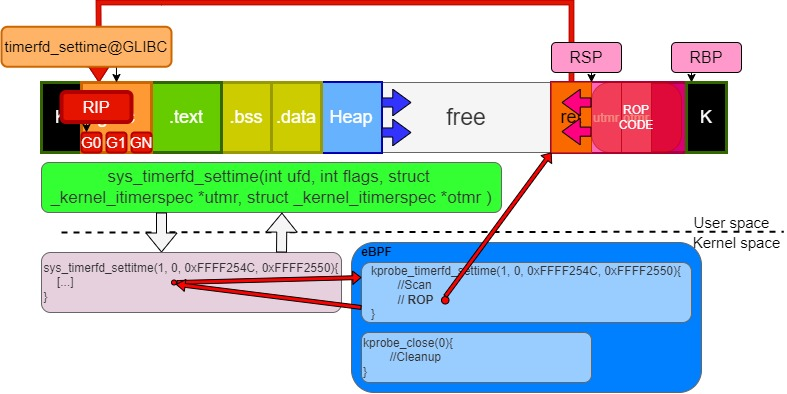
\includegraphics[width=15cm]{rop_evil_ebpf_2.jpg}
	\caption{Process memory after syscall exits and ROP code overwrites the stack.}
	\label{fig:rop_evil_ebpf_2}
\end{figure}

As we can see in the figure, the function has already exited, and ret has been popped into register rip. As we explained in section \ref{subsection:rop}, the attacker places in that position the address of the first ROP gadget. After that, the attacker can execute arbitrary code. Jeff Dileo, for instance, loads a malicious library into the process (we will do the same and explain this process in the next sections).

Once the attacker has finished executing the injected code, the stack must be restored to the original position so that the program can continue without crashing. A simplified view of this procedure consists of attaching a kprobe to a random system call (in this case, sys\_close()) so that, from the ROP code, we can alert the eBPF program when it is time to remove the ROP code and restore the original stack. Figure \ref{fig:rop_evil_ebpf_3} shows this final step:

\begin{figure}[H]
	\centering
	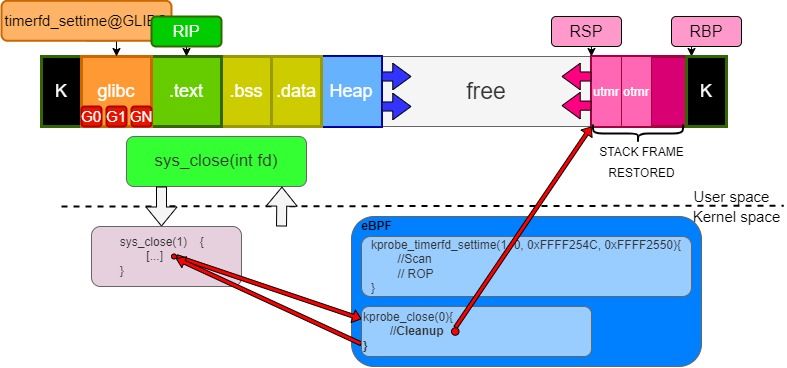
\includegraphics[width=15cm]{rop_evil_ebpf_3.jpg}
	\caption{Stack data is restored and program continues its execution.}
	\label{fig:rop_evil_ebpf_3}
\end{figure}

As we can see, eBPF writes back the original stack and thus the execution can continue. Note that, in practice, some final gadgets must also be executed in order to restore the state of rip and rsp, the stack data for this is written in the free memory zone, so that it does not need to be removed.


%TODO Eligible to writing more. This was merged with the explanation of each feature before, so it was more extense, but now it might need some more info??
\subsection{Bypassing hardening features in ELFs}
During section \ref{subsection:hardening_elf}, we presented multiple  security hardening measures that have been introduced to prevent common exploitation techniques (such as stack buffer overflows) and that nowadays can be incorporated, usually by default, in ELF binaries generated using modern compilers. We will now explore how to bypass these features, so that we can later design an injection technique that can target any process in the system, independently on whether it was compiled using these mitigations.

\textbf{Stack canaries}\\
Since stack canaries will be checked after the vulnerable function returns, an attacker seeking to overwrite the stack must ensure that the value of the canary remains constant. In the context of a buffer overflow attack, this can be achieved by leaking the value of the canary and incorporating it into the overflowing data at the stack, so that the same value is written on the same address\cite{canary_exploit}.

In our rootkit, unlike in the ROP technique presented in section \ref{subsection:rop_ebpf}, we will avoid overwriting the value of the saved rip in the stack completely. Therefore, as long as our eBPF program leaves all registers and stack data in the same state as before calling the function, we will not trigger any alerts.

\textbf{DEP/NX}\\
The only alternative for an attacker upon a non-executable stack is either injecting shellcode at any other executable memory address, or the use of advanced techniques like ROP that fully circumvent this mitigation since the data at the stack is not directly executed at any step.

In our rootkit, we will choose the first option, scanning the process virtual memory for an executable page where we will inject our shellcode. This process is usually known as finding 'code caves'.

\textbf{ASLR}\\
In order to bypass ASLR, attackers must take into account that, although the address at which, for instance, a library is loaded is random, the internal structure of the library remains unchanged, with all symbols in the same relative position, as figure \ref{table:aslr_offset} shows.

%TODO Add the .data section here
\begin{figure}[H]
	\centering
	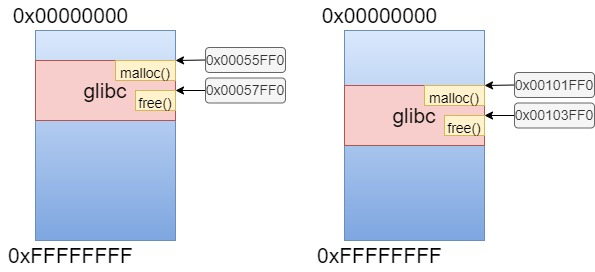
\includegraphics[width=13cm]{aslr_offset.jpg}
	\caption{Two runs of the same executable using ASLR, showing a library and two symbols.}
	\label{fig:alsr_offset}
\end{figure}

As we can observe in the figure, although glibc is loaded at a different base address each run, the offset between the functions it implements, malloc() and free(), remains constant. Therefore, a method for bypassing ASLR is to gather information about the absolute address of any symbol, which can then easily lead to knowing the address of any other if the attacker decompiles the executable and calculates the offset between a pair of addresses where one is known. This is the chosen method for our technique.

\textbf{PIE}\\
Similarly to ASLR, although the starting base address of each memory section is random, the internal structure of each section remains the same. Therefore, if an attacker is able to leak the address of some symbol in a section, and by knowing the offset at which it is located with respect to the base address of the section, then the address of any other symbol in the same section can be calculated\cite{pie_exploit}. This is the technique we will incorporate in our rootkit.

\textbf{RELRO}\\
If an executable was compiled using Partial RELRO, then the value of GOT can still be overwritten. If in turn it was compiled using Full RELRO, this stops any attempt of GOT hijacking, unless an attacker finds an alternative method for writing into the virtual memory of a process that bypasses the read-only flag. 

In our rootkit, we will directly write using eBPF the value of GOT if it was compiled with Partial RELRO, and use an alternative technique for writing into the virtual memory of a process whenever it was compiled using Full RELRO.


\subsection{Library injection via GOT hijacking} \label{subsection:got_attack}
Taking into account the background about stack attacks, ELF's lazy binding and hardening features for binaries we presented in section \ref{section:elf}, we will now present the exploitation technique incorporated in our rootkit to inject a malicious library into a running process. 

This attack is based on the possibility of overwriting the data at the GOT section. As we have mentioned previously, this section is marked as writeable if the program was compiled using Partial RELRO, meaning that we will be able to overwrite its value from an eBPF program using the helper bpf\_probe\_write\_user(). After modifying the value of GOT, a PLT stub will take the new value as the jump address (as we explained in section \ref{subsection:elf_lazy_binding}), effectively hijacking the flow of execution of the program. In the case that a program was compiled with Full RELRO (which will be the case of many programs running by default in a Linux system such as systemd), we will make use of the /proc filesystem for overwriting this value.

The rootkit will inject the library only after the second time that an specific syscall is called by a process, since the first time we will wait for the GOT address to be loaded by the dynamic linker. This is a necessary step because eBPF will need to validate that it really is the GOT section to overwrite.

This technique works both in compilers with low hardening fetaures by default (Clang) and also on a compiler with all of them active (GCC), see table \ref{table:compilers}. On each of the steps, we will detail the different existing methods depending on the compiler features.

For this research work, the rootkit is prepared to perform this attack on any process that makes use of either the system call sys\_openat or sys\_timerfd\_settime, which are called by the standard library glibc.

\textbf{Stage 1: eBPF tracing and scan the stack}\\
We load and attach a tracepoint eBPF program at the \textit{enter} position of syscall sys\_timerfd\_settime. Firstly we must ensure that the process calling the tracepoint is one of the processes to hijack.

We will then proceed with the stack scanning technique, as we explained in section \ref{subsection:bpf_probe_write_apps}. In this case, the algorithm will go as follows:
\begin{enumerate}
\item Take one of the syscall parameters and scan forward in the scan. For each iteration, we must check if the data at the stack corresponds to the saved rip:
\begin{enumerate}
\item Check that the previous instruction is a call instruction, by checking the instruction length and opcodes (call instructions always start with e8, and the length is 5 bytes, see figure \ref{fig:firstcall}).
\begin{figure}[H]
	\centering
	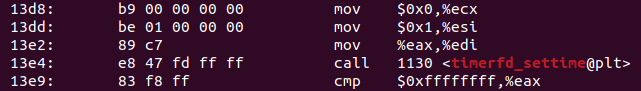
\includegraphics[width=13cm]{sch_firstcall.png}
	\caption{Call to the glibc function, using objdump}
	\label{fig:firstcall}
\end{figure}
\item Now that we know we localized a call instruction, we take the address at which it jumps. That should be an address in a PLT stub.
\item We analyze the instruction at the PLT stub. If the program was compiled with GCC, it will be an \textit{endbr64} instruction followed by the PLT jump instruction using the address at GOT (since it generates Intel CET-compatible programs, see table \ref{table:compilers}). Otherwise, if using Clang, the first instruction is the PLT jump.
%TODO Continue
\end{enumerate}
\end{enumerate}